\part{PDE}
\section{سری و تبدیل فوریه}
\subsection*{مقدمه}
در فصل ۱ هدف حل برخی از معادلات دیفرانسیل پاره ای است. برای این منظور سری و تبدیل فوریه به عنوان یک ابزار مهم استفاده می شوند. به همین دلیل، در این بخش ابتدا چند تعریف اساسی و مهم را در زمینه ی معادلات دیفرانسیل پاره ای ارائه می کنیم و سپس با سری و تبدیل فوریه آشنا می شویم. بعدا در بخش های ۲ و ۳ خواهیم دید که سری و تبدیل فوریه چگونه در حل برخی معادلات دیفرانسیل پاره ای به کار می روند.\\
\begin{definition}
 اگر 
$u:\R^n \to \R$
تابعی از متغیر های مستقل
$x_n,...,x_1$
باشد، یک معادله بین 
$u$
و 
$x_i$
 ها و مشتقات جزئی
 $u$
 نسبت به
 $x_i$
 ها را یک معادله دیفرانسیل با مشتقات جزئی یا معادلات دیفرانسیل پاره ای می نامیم.\\
\end{definition}
 به عنوان نمونه
 \begin{equation}
u+u_x+u_{xy}+uu_{yy}=x^2y
\end{equation}
\begin{equation}
u_{xx}+u_{yy}=0
\end{equation}
\begin{equation}
u_t=u_{xx}+uu_x
\end{equation}
\begin{equation}
u_x+u_{xxy}=0
\end{equation}
معادلات دیفرانسیل با مشتقات جزئی هستند.\\
\begin{definition}
 مرتبه معادله دیفرانسیل پاره ای عبارت از بزرگترین مرتبه مشتق جزئی ظاهر شده در آن است.
\end{definition}
  به عنوان نمونه معادله دیفرانسیل پاره ای (۴) یک معادله ی مرتبه ۳ است.\\
مرتبه نسبت به هر متغیر مستقل به طور مجزا نیز تعریف می شود. مثلا معادله ی 
$(4)$
 نسبت به 
$x$
مرتبه ۲ و نسبت به 
$y$
مرتبه ۱ است.\\

\begin{definition}
معادله دیفرانسیل پاره ای را همگن می گوییم اگر جمله ای که فقط وابسته به متغیر های مستقل است، نداشته باشد(برابر با صفر باشد).\\
\end{definition}
معادله
$(1)$
  ناهمگن و معادلات
$(4),(3),(2)$
 همگن هستند.\\
 
\begin{definition}
 یک معادله دیفرانسیل پاره ای را خطی می گوییم اگر ضریب
 $u$
 و مشتقات جزئی آن فقط تابعی از متغیر های مستقل باشند.
\end{definition}
  معادلات
 $(2)$
 و
 $(4)$
 خطی و معادلات 
 $(1)$
 و
 $(3)$
 به ترتیب به خاطر وجود جملات
 $uu_{yy}$
 و
 $uu_x$
 غیر خطی هستند.\\
\\
 در درس ریاضی مهندسی چند نمونه از معادلات خطی (ضریب ثابت) را بررسی می کنیم.
 
 این معادلات عبارتند از :
 \begin{enumerate}
 	\item 
 	\textbf{
 	معادله حرارت : 
 }
 	$u_t=\alpha u_{xx}$
 	\item
 	معادله موج (مدل سازی نوسان در یک طناب) : 
 	$u_{tt}=c^2u_{xx}$
 	\item
 	معادله ی لاپلاس (انتقال حرکت پایا در یک صفحه) : 
 	$u_{xx}+u_{yy}=0$
 	\item
 	معادله ی تیر :
 	$u_{tt}=au_{xxxx}$
 \end{enumerate}

نکته : هر مساله ی 
PDE
برای داشتن جواب یکتا، نسبت به متغیر به تعداد مرتبه آن شرط اولیه نیاز دارد.\\
به عنوان نمونه مسئله ی حرارت با داشتن یک شرط اولیه برای 
$t$
و دو شرط مرزی برای 
$x$
جواب یکتا دارد.\\
در ادامه ابتدا سری فوریه و سپس تبدیل فوریه را می بینیم.
\subsection*{مدل سازی مسائل حرارت، لاپلاس و موج}
\subsubsection{انتقال حرارت در یک میله ی فلزی}
انتقال حرارت در یک میله ی فلزی به طول $L$
را بررسی می کنیم. چگالی، ضریب هدایت و ظرفیت گرمایی فلز را به ترتیب برابر با $\rho$، $k$ و  $c_p$ در نظر می گیریم. همچنین فرض می کنیم که قطر میله نسبت به طول آن بسیار کوچک است و بنایراین تغییر دما در راستای شعاع میله وجود ندارد. در این صورت طبق قانون هدایت فوریه داریم:
\begin{figure}[H]
	\centering
	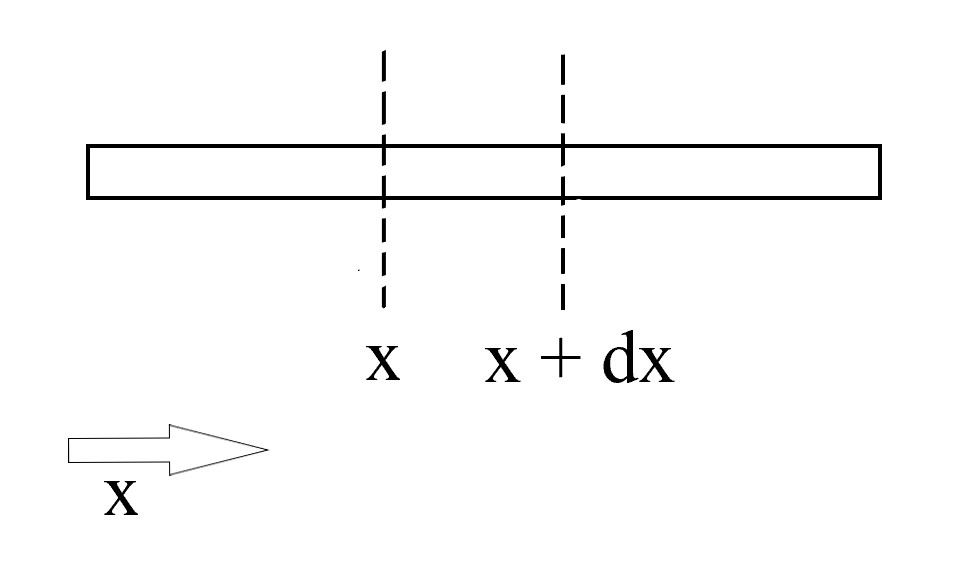
\includegraphics[width=0.275\textwidth]{im01.jpg}
	\caption*{شکل ۱: مدلسازی انتقال حرارت یک بعدی\\
		\large{
}
}
\end{figure}

\[(\left.KA\frac{\partial u}{\partial x}\right|_{x+\Delta x}-\left.KA\frac{\partial u}{\partial x}\right|_{x}) \cdot \Delta t=
	mc_p \cdot \Big(u(x,t+\Delta t)-u(x,t)\Big)\]
و
\[m=\rho \cdot \Delta v=\rho \cdot  A \cdot \Delta x\]
که در آن $u(x,t)$ دمای نقطه به طول $x$ در لحظه $t$ است. پس
\begin{alignat*}{1}
&\begin{cases}
\left.\frac{\partial u}{\partial x}\right|_{x+\Delta x}-\left.\frac{\partial u}{\partial x}\right|_{x} = \frac{\partial^2 u}{\partial x^2}  \cdot \Delta x\\
u(x,t+\Delta t)-u(x,t)=\frac{\partial u}{\partial t} \cdot \Delta t
\end{cases} 
\\& \Rightarrow 
K A \cdot \frac{\partial^2 u}{\partial x^2}  \Delta x \Delta t=c_p\rho A\frac{\partial u}{\partial t}\Delta t\Delta x
\\& \Rightarrow
\frac{\partial u}{\partial t}=\frac{k}{c_p\rho} \cdot \frac{\partial^2 u}{\partial x^2}
\end{alignat*}

پس اگر تعریف کنیم
$\alpha := \frac{k}{c_p\rho}$
متوجه می شویم که\\
\[u_t=\alpha u_{xx}\]
\[u(0,t)=u(L,t)=0\]
\[u(x,0)=f(x)\]
اگر هم این مسئله را در ۲ بعد بررسی کنیم، به دلیل وجود هدایت گرما در هر دو راستای $x$ و $y$ خواهیم داشت\\:
\begin{figure}[H]
	\centering
	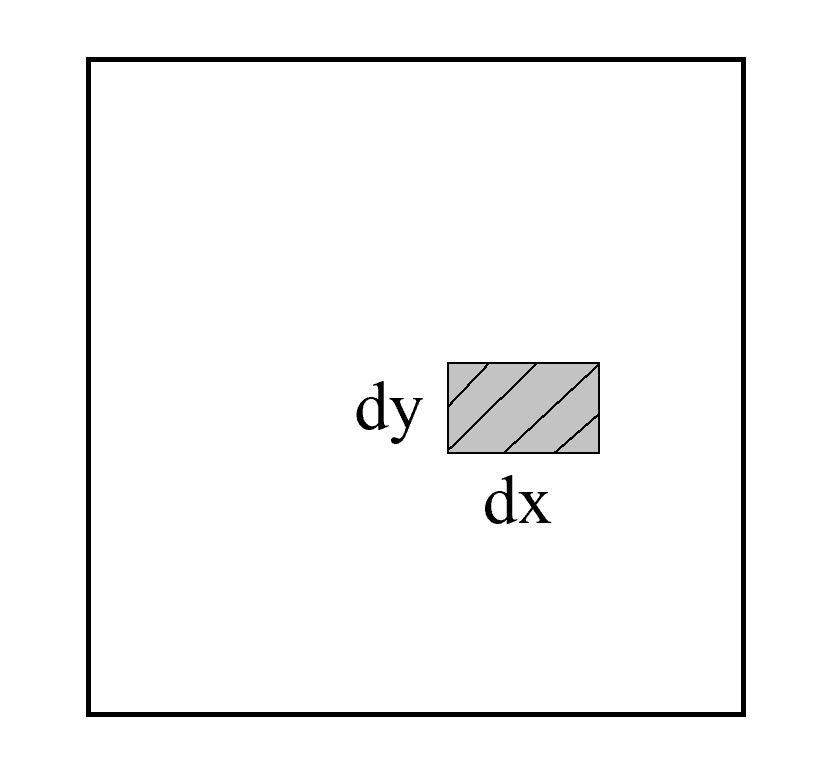
\includegraphics[width=0.275\textwidth]{im02.jpg}
	\caption*{شکل ۲: مدلسازی انتقال حرارت دو بعدی\\
		\large{
}
}
\end{figure}


\[\frac{\partial u}{\partial t}=\alpha(\frac{\partial^2 u}{\partial x^2}+\frac{\partial^2 u}{\partial y^2})\]
\subsubsection{
	معادله لاپلاس، انتقال حرارت پایا
	 \lr{(steady state)}
}
\begin{equation*}
	\begin{aligned}
	{} &\ \frac{\partial u}{\partial t}=0 \\
	&\ \frac{\partial u}{\partial t}=\alpha(\frac{\partial^2 u}{\partial x^2}+\frac{\partial^2 u}{\partial y^2}) \\
	&\ \Rightarrow \frac{\partial^2 u}{\partial x^2}+\frac{\partial^2 u}{\partial y^2}=0
	\end{aligned}
\end{equation*}
پس داریم
\begin{equation*}
\begin{aligned}
{} &\ 
u_{xx}+u_{yy}=0
\\
&\
u_x(0,y)=u_x(a,y)=0
\\
&\
u(x,0)=f(x)
\\
&\
u(x,b)=g(x)
\\
\end{aligned}
\end{equation*}



\subsubsection{موج (نوسان طناب)}
حال مدلسازی نوسان طناب یک بعدی را بررسی می کنیم. چنانچه، طناب دارای طول $L$، جرم $M$ و سختی $K$ باشد و $u(x,t)$ ارتفاع نقطه به طول $x$ در لحظه باشد، بر اساس قانون هوک داریم:
\begin{figure}[H]
	\centering
	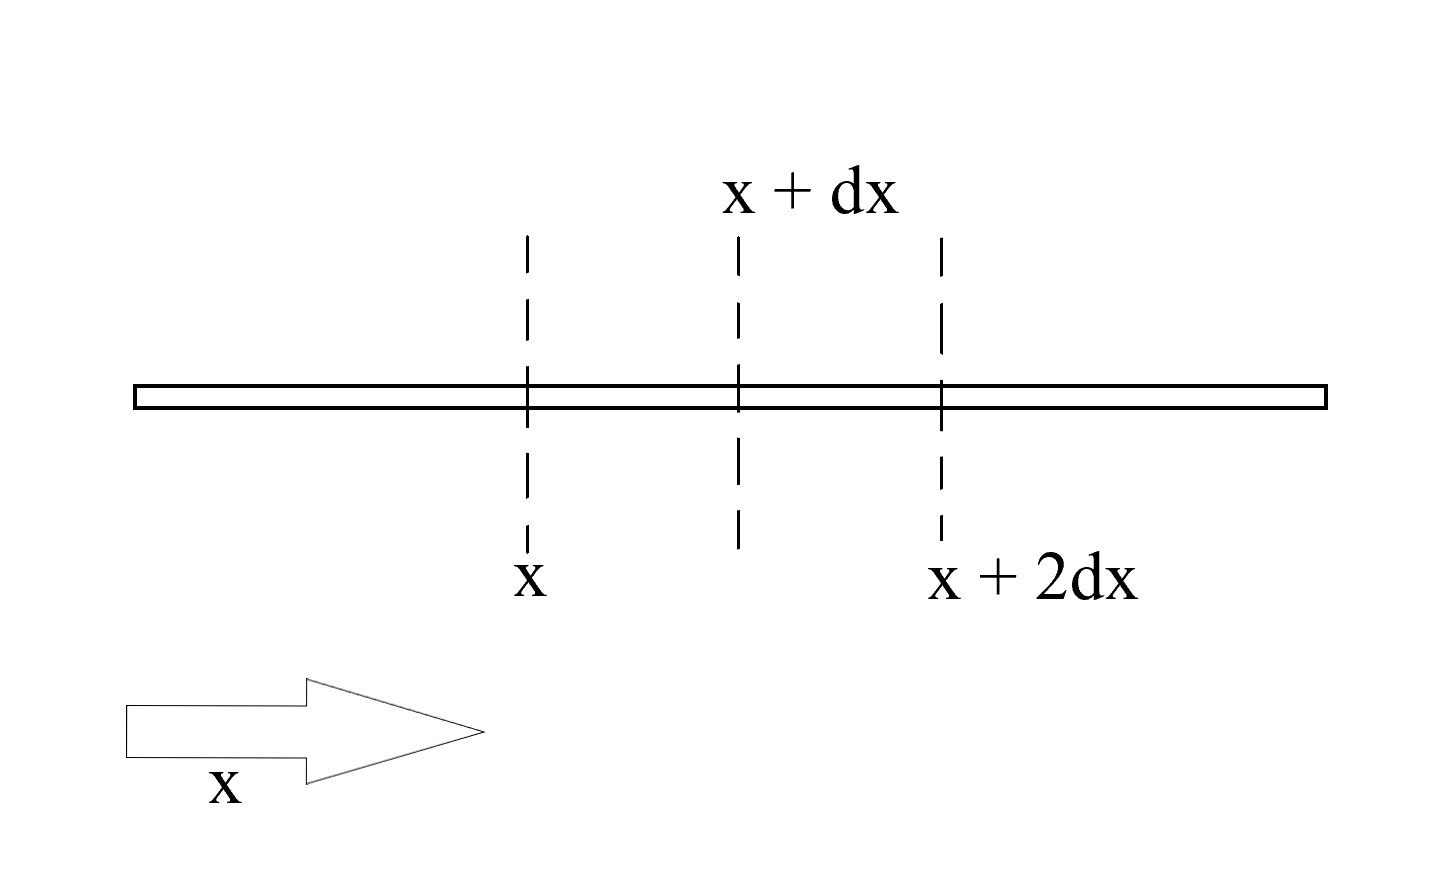
\includegraphics[width=0.275\textwidth]{im03.jpg}
	\caption*{شکل ۳: مدلسازی نوسان یک بعدی\\
		\large{
}
}
\end{figure}\\

 \[
 F=k[u(x+2\Delta x)-u(x+\Delta x)]-k[u(x+\Delta x)-u(x)]=ma=m\frac{\partial^2 u}{\partial t^2}
 \]
 همچنین، فرض می کنیم هر المان طناب با طول $dx$ دارای جرم $m$ و سختی $k$ باشد و کل طناب از $n$ المان تشکیل شود.
 \begin{figure}[H]
	\centering
	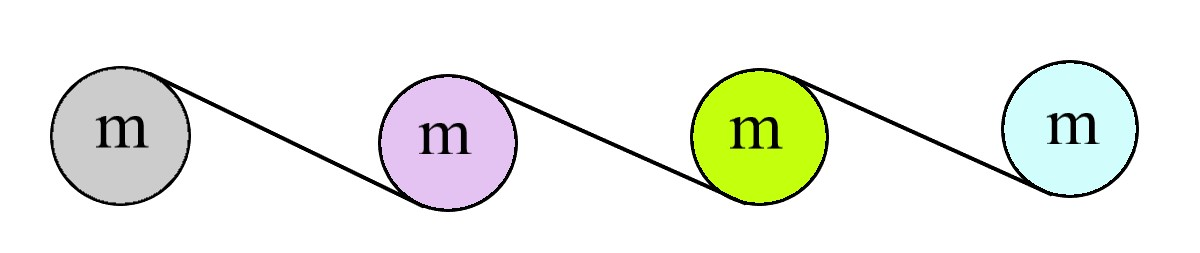
\includegraphics[width=0.275\textwidth]{im04.jpg}
	\caption*{شکل ۴: المان های مورد نیاز برای مدلسازی\\
		\large{
}
}
\end{figure}\\
 بنابراین، 
 $L=n\Delta x$
 و
 $M=nm$
 و
 $K=\frac{k}{n}$
 حال با توجه به رابطه قبلی داریم
 \begin{equation*}
 \begin{aligned}
 k\Big(u(x+{}&\ 2\Delta x,t)- 2u(x+\Delta x,t)+u(x,t)\Big)=m\frac{\partial^2 u}{\partial t^2}\\
 &\  \Rightarrow  u_{tt}=\frac{k}{m}u_{xx}(\Delta x)^2\\
 &\  \Rightarrow u_{tt}=\frac{k(\Delta x)^2}{m}u_{xx}\\ 
 &\ \Rightarrow u_{tt}=\frac{nK\frac{L^2}{K^2}}{\frac{M}{n}}u_{xx}\\
 &\  \Rightarrow u_{tt}=\frac{KL^2}{M}u_{xx} \\
 \end{aligned}
 \end{equation*}
تعریف می کنیم
$c^2 = \frac{KL^2}{M}$
.
پس داریم

\begin{equation*}
\begin{aligned}
{}&\ u_{tt}=c^2u_{xx} \\
&\ u(0,t)=u(L,t)=0 \\
&\ u(x,0)=f(x) \\
&\ u_t(x,0)=g(x) \\
\end{aligned}
\end{equation*}

اگر هم این مسئله را در ۲ بعد بررسی کنیم، خواهیم داشت\\
\begin{figure}[H]
	\centering
	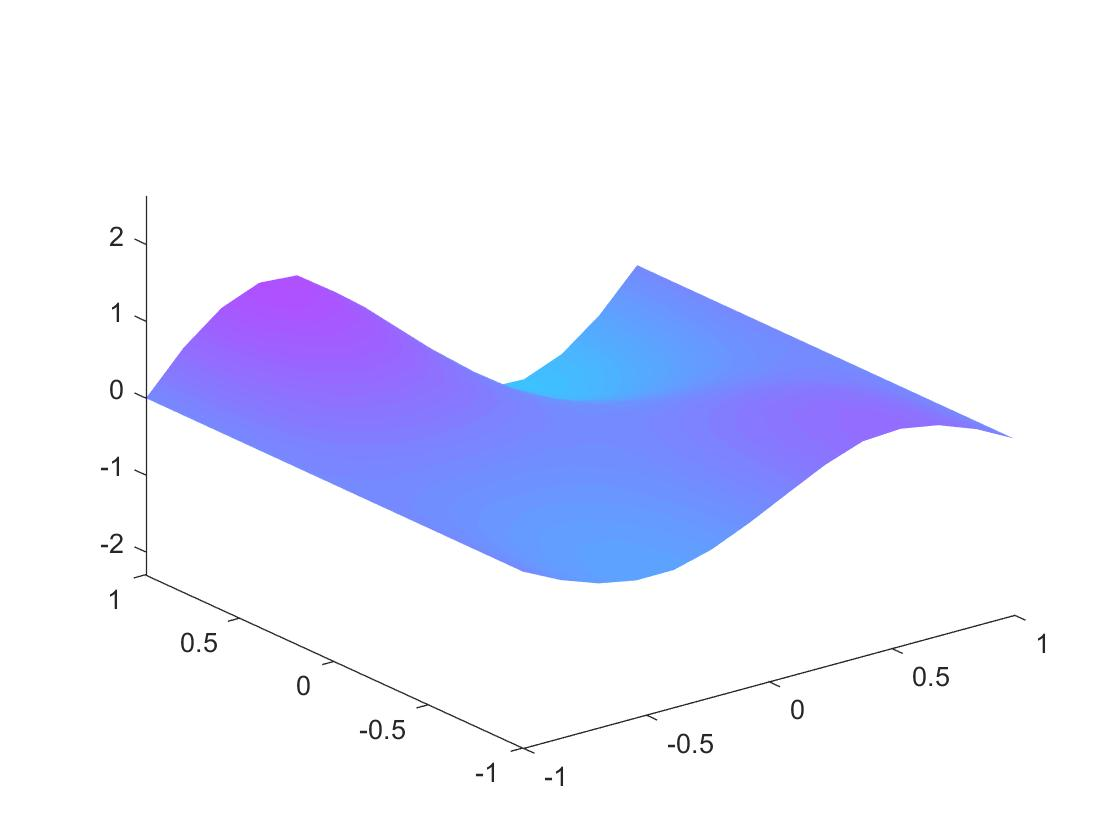
\includegraphics[width=0.275\textwidth]{im05.jpg}
	\caption*{شکل ۵: مدلسازی نوسان دو بعدی\\
		\large{
}
}
\end{figure}\\
\[
u_{tt}=c^2(u_{xx}+u_{yy})
\]

\subsection*{سری فوریه}
۱) تابع پیوسته و متناوب
$f$
 با دوره تناوب
 $2\pi$\\
 اگر 
 $f:\R\to\R$
 پیوسته و متناوب با دوره ی تناوب 
 $2\pi$
 باشد، ضرایب
 $a_k,a_0$
 و
 $b_k$
 موجودند به طوری که به ازای هر
 $x\in\R$
 داریم
 \begin{equation}
 f(x)=\int_{-\pi}^{\pi}{\frac{a_0}{2}dx}+\sum_{k=1}^\infty {\int_{-\pi}^{\pi}{a_kcos(kx)dx}}+\sum_{k=1}^\infty{\int_{-\pi}^{\pi}{b_ksin(kx)dx}}
 \end{equation}
 همچنین داریم
 \begin{equation}
 a_0=\frac{1}{\pi}\int_{-\pi}^{\pi} {f(x)dx}
 \end{equation}
 \begin{equation}
 a_k=\frac{1}{\pi}\int_{-\pi}^{\pi} {f(x)cos(kx)dx}
 \end{equation}
  \begin{equation}
 b_k=\frac{1}{\pi}\int_{-\pi}^\pi {f(x)sin(kx)dx}
 \end{equation}
 
 
 \begin{proof}
  برای محاسبه ضریب
 $a_0$
 ، کافی است از طرفین 
 $(5)$
 در بازه ی
 $[-\pi,\pi]$
 انتگرال بگیریم : 
 \[
 \int_{-\pi}^\pi {f(x)dx}=\int_{-\pi}^\pi{\frac{a_0}{2}}dx+\sum_{k=1}^\infty a_k{int_{-\pi}^\pi{cos(kx)dx}}+\sum_{k=1}^\infty b_k{int_{-\pi}^\pi{sin(kx)dx}}
 \]
 همچنین داریم :
 \[
 \int_{-\pi}^\pi{cos(kx)dx}=\left.\frac{sin(kx)}{k}\right |_{-\pi}^\pi=0
 \]
 \[
  \int_{-\pi}^\pi{sin(kx)dx}=0
 \]
 دقت کنید که دلیل رابطه آخر این است که
 $sin(kx)$
 تابعی فرد است و بازه انتگرال گیری متقارن است. بنابراین داریم
 \[
  f(x)=\frac{a_0}{2}(2\pi)+0+0\Rightarrow  a_0=\frac{1}{\pi}\int_{-\pi}^\pi {f(x)dx}
 \]
 حال برای محاسبه ضرایب 
 $a_j$
 ، ابتدا طرفین تساوی 
 $(5)$
 را در 
 $cos(jx)$
 ضرب می کنیم و سپس در بازه ی 
 $[-\pi,\pi]$
 انتگرال می گیریم :
 \begin{equation*}
 \begin{aligned}
 \int_{-\pi}^\pi{f(x)cos(jx)dx} {} &\ =\frac{a_0}{2}\int_{-pi}^\pi{cos(jx)dx}+\sum_{k=1}^\infty{\int_{-\pi}^\pi{cos(kx)cox(jx)dx}} \\
 &\ +\sum_{k=1}^\infty{a_k\int_{-\pi}^\pi{cos(kx)cox(jx)dx}} \\
 &\ +\sum_{k=1}^\infty{b_k\int_{-\pi}^\pi{cos(kx)sin(jx)dx}} \\
 \end{aligned}
 \end{equation*}
 از طرفی برای هر عدد صحیح
 $j\ne0$
 داریم
 \[
 \int_{-\pi}^\pi{cos(jx)dx}=\left.{\frac{sin(kx)}{k}}\right |_{-\pi}^\pi=0
 \]
 وبرای هر 
 $j,k$
 صحیح، با توجه به فرد بودن تابع
 $sin(kx)cos(jx)$
 داریم
 \[
 \int_{-\pi}^\pi{sin(kx)cos(jx)dx}=0
 \]
 و همچنین داریم
\begin{align*}
 \int_{-\pi}^\pi{cos(kx)cox(jx)dx}&=
\begin{cases}
\int_{-\pi}^\pi{\frac{1}{2}\Big[cos\big((k+j)x\big)+cos\big((k-j)x\big)\Big]} &\mbox{if } k\ne j\\
\int_{-\pi}^\pi{\frac{1+cos(2jx)}{2}dx}   
	&\mbox{if } k=j\\
\end{cases}
\\
&=\begin{cases}
0 &\mbox{if } k\ne j
\\
\pi &\mbox{if } k=j
\end{cases}
\end{align*}
 و بنابراین متوجه می شویم که برای هر 
 $j\in\N$
 داریم
 \[
 \int_{-\pi}^\pi{f(x)cos(jx)dx} {} = 0+a_j\times\pi+0\Rightarrow a_j=\frac{1}{\pi}\int_{-\pi}^\pi{f(x)cos(jx)dx}
 \]
 به طور مشابه با ضرب طرفین
 $(5)$
 در
 $sin(jx)$
 و انتگرال گیری در بازه
 $[-\pi,\pi]$
 می توان نشان داد که برای هر 
 $j\in\N$
 ،
 $b_j=\frac{1}{\pi}\int_{-\pi}^\pi{f(x)sin(jx)dx}$
 است.\\
 \end{proof}
 
\begin{example}
 
 سیگنال مثلثی
\begin{align*}
 &f(x)=
 \begin{cases}
 \pi-x &\mbox{if  } { 0\le x\le \pi}
 \\
 \pi+x &\mbox{if  }  {-\pi\le x \le 0}
 \end{cases}
 &f(x+2\pi)=f(x)
\end{align*}

\hrulefill

حل- 
 \begin{equation*}
 \begin{aligned}
 a_0 {} &\ = \frac{1}{\pi}\int_{-\pi}^\pi{f(x)dx}\\
 &\ =\frac{1}{\pi}\left(\int_{-\pi}^0{\pi-x \, dx}+\int_0^\pi{\pi+x \, dx}\right)\\
 &\ =\frac{1}{\pi}\left(
 \left.{\frac{(\pi+x)^2}{2}}\right |_{-\pi}^0
 +
  \left.{\frac{-(\pi-x)^2}{2}}\right |_0^\pi
 \right)\\
 &\ = \frac{1}{\pi}\left(
 \frac{\pi^2}{2}-0+0+\frac{\pi^2}{2}
 \right)= \pi
 \\\\
  a_k {} &\ = \frac{1}{\pi}\int_{-\pi}^\pi{f(x)cos(kx)dx}\\
 &\ = \frac{1}{\pi}\left(
 \int_{-\pi}^{0}{(\pi+x)cos(kx) dx} +\int_{0}^{\pi}{(\pi-x)cos(kx)dx}
 \right)\\
 &\ = \frac{1}{\pi}\left(
 \int_{-\pi}^{0}{xcos(kx) dx} -\int_{0}^{\pi}{(xcos(kx)dx}
 \right)
 +
 \int_{-\pi}^{\pi}{cos(kx)dx}
 \end{aligned}
 \end{equation*}

 که در آن 
 \begin{alignat*}{3}
 \int_{-\pi}^{0}{xcos(kx)dx}
 = & \left.{\frac{xsin(kx)}{k}}\right |_{-\pi}^{0} & -\int_{-\pi}^{0}{\frac{sin(kx)}{k}dx}
 &= \frac{1-(-1)^k}{k^2}
\\
 \int_{0}^{\pi}{xcos(kx)dx}
 = & \left.{\frac{xsin(kx)}{k}}\right |_{0}^{\pi} & -\int_{0}^{\pi}{\frac{sin(kx)}{k}dx}
 &=\frac{(-1)^k-1}{k^2}
 \\
 \int_{-\pi}^{\pi}{cos(kx)dx}=& 0
 \end{alignat*}

 بنابراین
 \[
 a_k=\frac{1}{\pi}\frac{2}{k^2}\left(1-(-1)^k\right)=
 \begin{cases}
 0 &\mbox{if } k=2n\\
 \frac{4}{\pi(2n-1)^2} &\mbox{if } k=2n-1
 \end{cases}
 \]
 و
\begin{equation*}
	\begin{aligned}
	b_k {} &\ = \frac{1}{\pi}\int_{-\pi}^{\pi}{f(x)sin(kx)dx}\\
	&\ = \frac{1}{\pi}\left(
	\int_{-\pi}^{0}{(\pi+x)sin(kx)dx}+\int_{0}^{\pi}{(\pi-x)sin(kx)dx}
	\right)\\
	&\ = \frac{1}{\pi}\left(\int_{-\pi}^{0}{xsin(kx)dx}-\int_{0}^{\pi}{xsin(kx)dx} \right)+\int_{-\pi}^{\pi}{sin(kx)dx}
	\end{aligned}
\end{equation*}
که
\begin{alignat*}{2}
{} &\ \int_{-\pi}^{0}{xsin(kx)dx}
	=&\left.{-\frac{xcos(kx)}{k}}\right |_{-\pi}^{0} 
	&+\int_{-\pi}^{0}{\frac{cos(kx)}{k}dx}=\frac{\pi(-1)^{k+1}}{k}\\
&\ \int_{0}^{\pi}{xsin(kx)dx}
	=&\left.{-\frac{xcos(kx)}{k}}\right |_{0}^{\pi} 
	&+\int_{0}^{\pi}{\frac{cos(kx)}{k}dx}=\frac{\pi(-1)^{k+1}}{k}\\
&\ \int_{-\pi}^{\pi}{sin(kx)dx}=0
\end{alignat*}

پس 
$b_k=0$
است. پس\\
\[f(x)=\frac{\pi}{2}+\sum_{n=1}^{\infty}{\frac{4}{n(2n-1)^2}}cos(2n-1)x\]

\end{example}
\hrulefill

*توجه : نمودار 
$f(x)$
در مثال ۱ بصورت 
\begin{figure}[H]
	\centering
	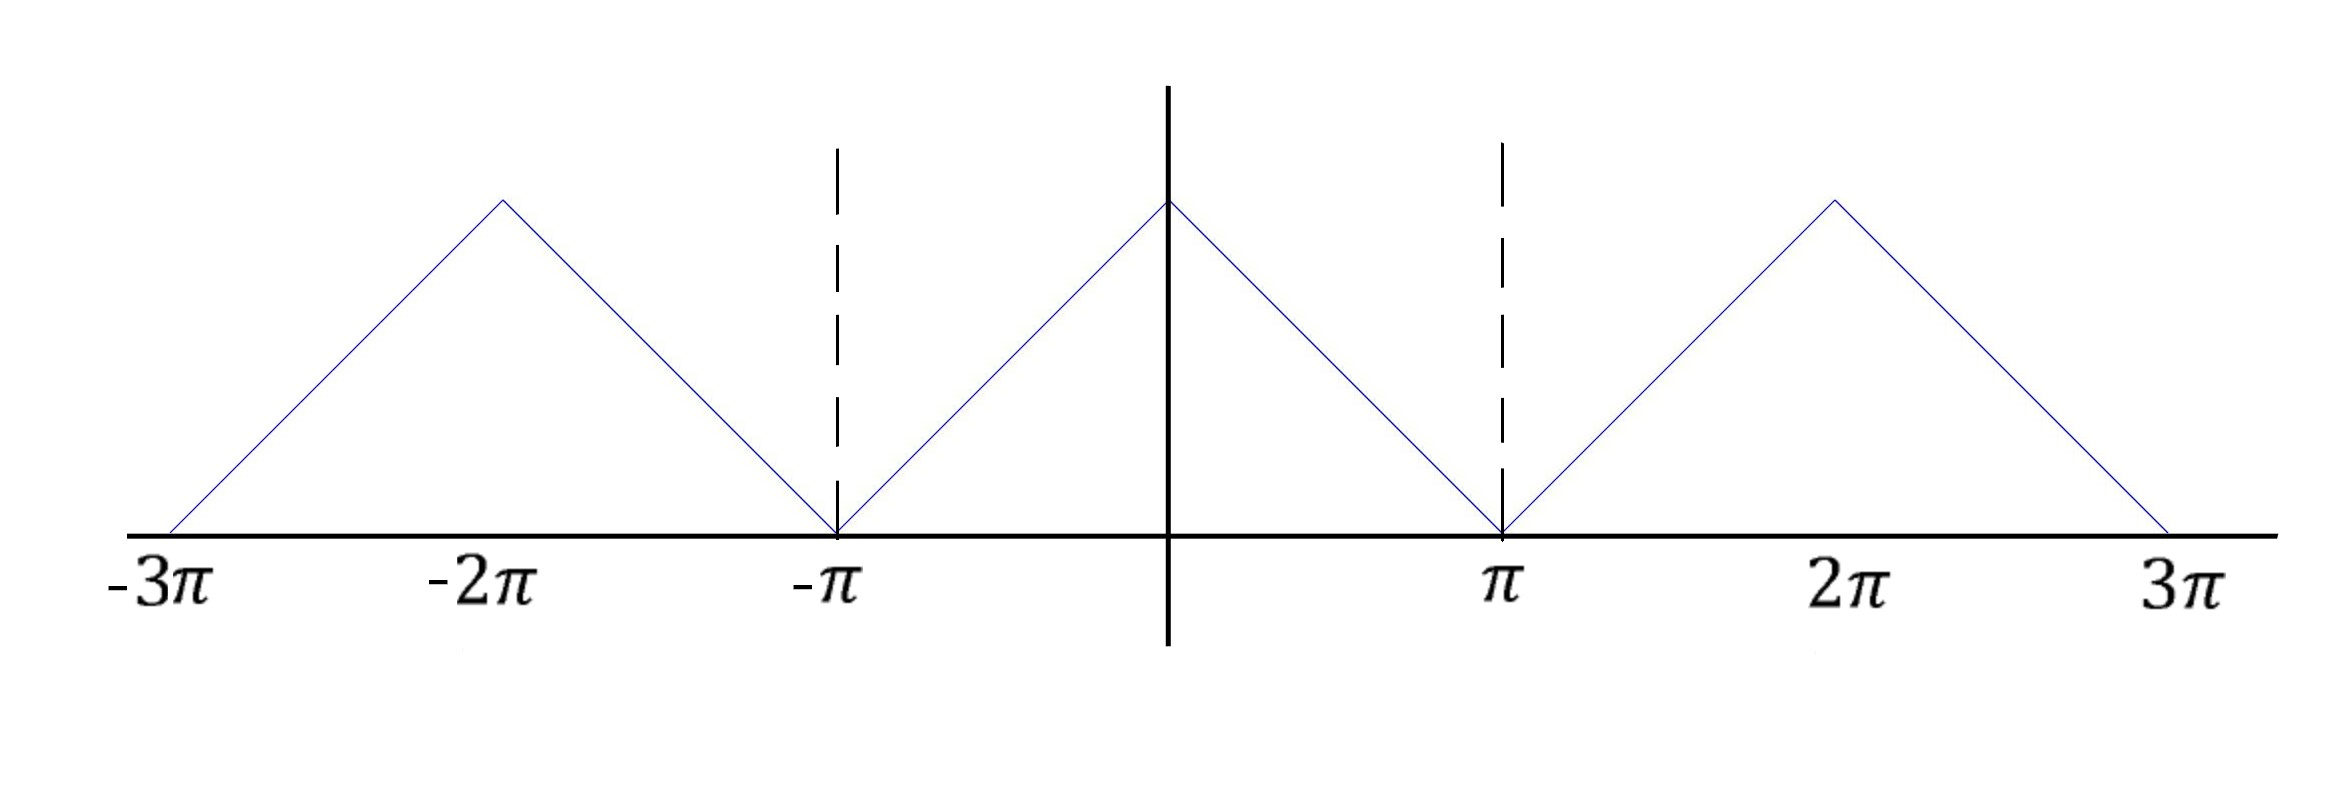
\includegraphics[width=0.275\textwidth]{im06.jpg}
	\caption*{شکل ۶: نمودار موج مثلثی\\
		\large{
}
}
\end{figure}
است. بنابراین 
$f(x)$
تابعی زوج است و در رابطه 
$(8)$
از زوج بودن 
$f$
و فرد بودن تابع
$sin(kx)$
نتیجه می شود که 
$b_k=0$.
پس توجه به زوج یا فرد بودن سیگنال 
$f(x)$
محاسبات ضرایب سری فوریه را ساده می کند. بعدا در مورد این نکته مفصل صحبت می کنیم.\\
توجه- اگر تابع 
$f(x)$
پیوسته و با دوره تناوب 
$2\pi$
بوده و در نقطه ی 
$x_0$
دارای ناپیوستگی نوع اول باشد، آنگاه سری فوریه ی
$f$
در
$x_0$
به میانگین حد چپ و راست همگراست.\\

\hrulefill

\begin{example}
سری فوریه ی تابع
$f(x)$
با ضابطه ی زیر را بدست آورید.
\begin{align*}
&f(x)=
\begin{cases}
0 &\mbox{if } 0\le x\le \pi
\\
\pi &\mbox{if } -\pi\le x \le 0
\end{cases}
& f(x+2\pi)=f(x)
\end{align*}
\hrulefill
\\
حل-
\begin{equation*}
\begin{aligned}
{} &\ a_0=\frac{1}{\pi}\int_{-\pi}^{\pi}{f(x)dx}=\frac{1}{\pi}\int_{0}^{\pi}{\pi dx}=\pi\\
&\ a_k=\frac{1}{\pi}\int_{-\pi}^{\pi}{f(x)cos(kx)dx}=\frac{1}{\pi}\int_{0}^{\pi}{\pi cos(kx) dx}=0\\
&\ b_k=\frac{1}{\pi}\int_{-\pi}^{\pi}{f(x)sin(kx)dx}=\frac{1}{\pi}\int_{0}^{\pi}{\pi sin(kx) dx}=\frac{1-(-1)^k}{k}\\
\end{aligned}
\end{equation*}

\end{example}
\hrulefill
حال در 
$x=0$
که نقطه ناپیوستگی است، داریم
$f^+(0)=\pi , f^-(0)=0$
و  سری فوریه در این نقطه به
$\frac{\pi}{2}=\frac{f^+(0)+f^-(0)}{2}$
همگراست.\\
\begin{example}
تابع زیر را در نظر بگیرید.
\begin{align*}
&f(x)=
\begin{cases}
-\pi &\mbox{if } -\pi\le x\le 0
\\
x &\mbox{if } 0\le x \le \pi
\end{cases}
& f(x+2\pi)=f(x)
\end{align*}
\hrulefill
\\
الف) سری فوریه ی تابع 
$f(x)$
را به دست آورید.\\
ب) نشان دهید 
$\sum_{k=1}^{\infty}{\frac{1}{(2k+1)^2}}=\frac{\pi^2}{8}$
\end{example}
حل-
\begin{equation*}
	\begin{aligned}
		a_0 {}
		&\
		=\frac{1}{\pi}\int_{-\pi}^{\pi}{f(x)dx}\\
		&\
		=\frac{1}{\pi}\left(\int_{-\pi}^{0}{\pi \, dx}+\int_{0}^{\pi}{x \, dx}\right)=\frac{1}{\pi}\left(\pi^2+\frac{\pi^2}{2}\right)=\frac{3\pi^2}{2}
	\end{aligned}
\end{equation*}
\begin{equation*}
	\begin{aligned}
		a_k {} &\
		=\frac{1}{\pi}\int_{-\pi}^{\pi}{f(x)dx} \\
		&\
		=\frac{1}{\pi}\left(\int_{-\pi}^{0}{\pi cos(kx)dx}+\int_{0}^{\pi}{x cos(kx)dx}\right)
		&\
		=\frac{1}{\pi}\left(-\int_0^\pi{\frac{sin(kx)}{x}dx}\right)=\frac{(-1)^k-1}{k^2\pi}
	\end{aligned}
\end{equation*}
\begin{equation*}
	\begin{aligned}
		b_k {} &\
		=\frac{1}{\pi}\int_{-\pi}^{\pi}{f(x)cos(kx)dx}\\
		&\
		=\frac{1}{\pi}\left(\int_{-\pi}^{0}{\pi sin(kx)dx}+\int_{0}^\pi{xsin(kx)dx}\right)\\
		&\
		=\frac{1}{\pi}\left(\frac{\pi\left((-1)^k-1\right)}{k}-\left.{\frac{xcos(kx)}{k}}\right |_0^\pi+\int_0^\pi{\frac{cos(kx)}{k}dx}\right)\\
		&\
		=\frac{1}{\pi}\left(\frac{\pi\left((-1)^k-1\right)}{k}-\frac{\pi(-1)^k}{k}+0\right)=-\frac{1}{k}
	\end{aligned}
\end{equation*}
پس در نقاط پیوستگی 
$f$
داریم
\[
f(x)=\frac{3\pi}{4}+\sum_{k=1}^\infty{\frac{(-1)^k-1}{k^2\pi}cos(kx)}+\sum_{k=1}^\infty{-\frac{1}{k}sin(kx)}
\]
و در نقاط ناپیوستگی 
$f$
شامل
$x_0=2k\pi$
داریم 
$cos(kx_0)=1,sin(kx_0)=0$
پس در این نقطه داریم
\begin{equation}
	\text{سری فوریه}=
	\frac{3\pi}{4}+\sum_{k=1}^\infty{\frac{(-1)^k-1}{k^2\pi}}
\end{equation}
همچنین 
$f^-(x_0)=\pi$
و
$f^+(x_0)=0$
و بنابراین 
\begin{equation}
	\text{سری فوریه}=
	\frac{0+\pi}{2}=\pi/2
\end{equation}
و از ترکیب تساوی
$(9)$
و
$(10)$
نتیجه می شود که
\[
\frac{3\pi}{4}+\sum_{k=1}^\infty{\frac{(-1)^k-1}{k^2\pi}}=\frac{\pi}{2}\Rightarrow
\sum_{k=1}^\infty{\frac{2}{(2k-1)^2\pi}}=\frac{\pi}{4}\Rightarrow
\sum_{k=1}^\infty{\frac{1}{(2k-1)^2}}=\frac{\pi^2}{8}
\]
۲) تابع متناوب
$f$
با دوره تناوب
$2L$\\
اگر
$f:\R\to\R$
متناوب با دوره ی تناوب 
$2L$
باشد، ضرایب 
$a_k,a_0$
و
$b_k$
موجودند به طوری که\\
الف) در نقاط پیوستگی 
$x$
\[
f(x)=\frac{a_0}{2}+\sum_{k=1}^\infty{a_kcos\left(\frac{k\pi}{L}\right)dx}+\sum_{k=1}^\infty{b_ksin\left(\frac{k\pi}{L}\right)dx}
\]
ب) و در نقاط ناپیوستگی نوع اول
$\tilde{x}$
\[
\frac{f^-(x_0)+f^+(x_0)}{2}=\frac{a_0}{2}+\sum_{k=1}^\infty{a_kcos\left(\frac{k\pi}{L}x\right)dx}+\sum_{k=1}^\infty{b_ksin\left(\frac{k\pi}{L}x\right)dx}
\]
همچنین داریم
\[
a_0=\frac{1}{L}\int_{-L}^L{f(x)dx}
\]
\[
a_k=\frac{1}{L}\int_{-L}^L{f(x)cos\left(\frac{k\pi}{L}x\right)dx}
\]
\[
b_k=\frac{1}{L}\int_{-L}^L{f(x)sin\left(\frac{k\pi}{L}x\right)dx},
\]
اثبات- برای اثبات کافی است با یک تغییر متغیر خطی مناسب دوره تناوب را به
$2\pi$
تبدیل کنیم. قرار می دهیم
$t=\frac{\pi}{L}x$.
در این صورت داریم
\[
f(x)=f(\frac{L}{\pi}t)=g(t)
\]
و 
$g$
دارای دوره تناوب 
$2\pi$
است، زیرا :
\[
g(t+2\pi)=f\left(\frac{L}{\pi}\left(t+2\pi\right)\right)=f\left(\frac{L}{\pi}t+2L\right)=f\left(\frac{L}{\pi}t\right)=g(t)
\]
بنابراین
$g(t)$
دارای سری فوریه ای به فرم
\begin{equation}
	g(t)=\frac{a_0}{2}+\sum_{k=1}^\infty{a_kcos(kt)}+\sum_{k=1}^\infty{b_ksin(kt)}
\end{equation}
است که در آن
\[
a_0=\frac{1}{\pi}\int_{-\pi}^\pi{g(t)dt}
\]
\[
a_k=\frac{1}{\pi}\int_{-\pi}^\pi{g(t)cos(kt)dt)}
\]
\[
b_k=\frac{1}{\pi}\int_{-\pi}^\pi{g(t)sin(kt)dt}
\]
است.\\
حال کافی است در
$(11)$
متغیر
$t$
را دوباره به 
$x$
تبدیل کنیم. بنابراین
\[
f(x)=g(t)=\frac{a_0}{2}+\sum_{k=1}^\infty{a_kcos\left(\frac{k\pi}{L}\right)dx}+\sum_{k=1}^\infty{b_ksin\left(\frac{k\pi}{L}\right)dx}
\]
\[
a_0=\frac{1}{\pi}\int_{-\pi}^\pi{g(t)dt}=
\frac{1}{\pi}\int_{-L}^L{g\left(\frac{\pi}{L}x\right)\frac{\pi}{L}x \, dx}=\frac{1}{\pi}\int_{-L}^L{\frac{\pi}{L}f(x)dx}=
\frac{1}{L}\int_{-L}^L{f(x)dx}
\]
و به طور مشابه روابط
$a_k$
و
$b_k$
نیز اثبات می شود.\\
مثال- سری فوریه ی همگرا به تابع زیر را بدست آوردید و در نقاط ناپیوستگی مقدار همگرایی را به دست آورید.
\begin{equation*}
	\begin{gathered}
	x \quad \text{if } -1\le x\le 1
	\\
	 f(x+2)=f(x)
	\end{gathered}
\end{equation*}
حل-
\begin{equation*}
	\begin{aligned}
		{} &\
		2L=2\Rightarrow L=1
		\\ &\
		a_0=\frac{1}{1}\int_{-1}^1{f(x)dx}=\int_{-1}^1{x \, dx}=0
		\\ &\
		a_k=\frac{1}{1}\int_{-1}^1{f(x)cos(k\pi x)dx}=\int_{-1}^1{xcos(k\pi x)dx}=0 
		\\ &\ \begin{aligned}
			b_k {} &\
			=\frac{1}{1}\int_{-1}^1{f(x)sin(k\pi x)dx}=\int_{-1}^1{sin(k\pi x)dx}=\left. {-\frac{xcos(k\pi x)}{k\pi}}\right |_{-1}^1+\int_{-1}^1{\frac{cos(k\pi x)}{k}dx}
			\\ &\ 
			= \frac{(-1)^{k+1)}}{k\pi}+\frac{(-1)^{k+1)}}{k\pi}+0=\frac{2(-1)^{k+1)}}{k\pi}
		\end{aligned}
	\end{aligned}
\end{equation*}
پس در نقاط پیوستگی داریم
\[
f(x)=\sum_{k=1}^{\infty}{\frac{2(-1)^{k+1}}{k\pi}sin(k\pi x)}
\]
و در نقاط ناپیوستگی
$\tilde{x}=n$
داریم 
\[
\forall k\in\N: sin(k\pi \tilde{x})=0\Rightarrow f(\tilde{x})=0
\]
همچنین داریم
$f^-\left(\tilde{x}\right)=-1 ,f^-\left(\tilde{x}\right)=1$
پس
\[
f\left(\tilde{x}\right)=\frac{f^-\left(\tilde{x}\right)+f^+\left(\tilde{x}\right)}{2}
\]
* توجه - همان طور که در مثال قبل دیدیم، فرد بودن تابع 
$f$
باعث شد که ضرایب
$a_0$
و 
$a_k$
سری فوریه صفر شوند. به طور کلی زوج یا فرد بودن تابع محسابات ضرایب سری فوریه را کوتاه تر می کند. در ادامه این بحث را دقیق تر بررسی می کنیم.\\
* تابع زوج 
$f$
با دوره تناوب
$2L$
\begin{equation*}
	\begin{aligned}
		{} &\
		a_0=\frac{1}{L}\int_{-L}^L{f(x)dx}=\frac{2}{L}\int_{0}^L{f(x)dx}
		\\ &\
		a_k=\frac{1}{L}\int_{-L}^L{f(x)cos\left(\frac{k\pi}{L}x\right)dx}=\frac{2}{L}\int_{0}^L{f(x)cos\left(\frac{k\pi}{L}x\right)dx}
		\\ &\
		b_k=\frac{1}{L}\int_{-L}^L{f(x)sin\left(\frac{k\pi}{L}x\right)dx}=0
	\end{aligned}
\end{equation*}
بنابراین روابط فوق برای توابع زوج محاسبه ی ضریب سری فوریه را ساده می کنند.\\
* تابع فرد 
$f$
با دوره تناوب 
$2L$
\begin{equation*}
	\begin{aligned}
		{} &\
		a_0=\frac{1}{L}\int_{-L}^L{f(x)dx}=0
		\\ &\
		a_k=\frac{1}{L}\int_{-L}^L{f(x)cos\left(\frac{k\pi}{L}x\right)dx}=0
		\\ &\
		b_k=\frac{1}{L}\int_{-L}^L{f(x)sin\left(\frac{k\pi}{L}x\right)dx}=\frac{2}{L}\int_{0}^L{f(x)sin\left(\frac{k\pi}{L}x\right)dx}
	\end{aligned}
\end{equation*}
مثال- سری فوریه ی تابع
$f$
با ضابطه ی زیر را بدست آورید.
\begin{equation*}
	\begin{gathered}
		f(x) =
		\begin{cases}
			x       & \quad \text{if }\;\; 0\le x\le 2 \\
			-x  & \quad \text{if }\;\; -2\le x< 0
		\end{cases}\\
	f(x+4)=f(x)
	\end{gathered}
\end{equation*}
حل- تابع زوج است و بنابراین برای محاسبه ی ضرایب سری فوریه داریم :
\begin{equation*}
	\begin{aligned}
		{} &\
		2L=4\Rightarrow L=2
		\\ &\
		a_0=\frac{2}{2}\int_0^2{f(x)dx}=\frac{2}{2}\int_0^2{2 \, dx}=2
		\\ &\
		\begin{aligned}
			a_k {} &\
			= \frac{2}{2}\int_0^2{f(x)cos\left(\frac{k\pi}{2}x\right)dx}=
			\frac{2}{2}\int_0^2{x\,cos\left(\frac{k\pi}{2}x\right)dx}
			\\ &\
			=\left.{\frac{2}{k\pi}x \, sin\left(\frac{k\pi}{2}x\right)}\right |_0^2-\int_0^2{\frac{2}{k\pi} sin\left(\frac{k\pi}{2}x\right)}
			\\ &\
			0+\frac{4}{k^2\pi^2}\left.{cos\left(\frac{k\pi}{2}x\right)} \right |_0^2
			=\frac{4}{k^2\pi^2}\left( (-1)^k-1\right)
		\end{aligned}
	\\ &\
	b_k = 0
	\\ &\
	\implies f(x)=1+\sum_{k=1}^\infty{\frac{4}{k^2\pi^2}\left( (-1)^k-1\right)cos\left( \frac{k\pi}{2}x\right)}
	\end{aligned}
\end{equation*}
*کاربرد سری فوریه در حل معادلات پاره ای\\
در بخش دوم خواهیم دید که در حل معادلات پاره ای با استفاده از روش جداسازی لازم است برای تابع داده شده ی
$f(x)$
سری فوریه ای به دست آوریم که در بازه ی
$[0,L]$
به آن همگرا باشد. در  بعضی از موارد لازم است این سری فوریه فقط شامل جملات سینوسی یا کسینوسی باشد. نحوه ی محاسبه چنین سری فوریه ای را در ادامه می بینیم.\\
۱)سری فوریه ی کسینوسی که در بازه ی
$[0,L]$
به 
$f(x)$
همگراست.\\
با توجه به اینکه می خواهیم سری فوریه فقط شامل جملات کسینوسی باشد، لازم است یک گسترش زوج برای 
$f(x)$
در نظر بگیریم که در بازه ی
$[0,L]$
با 
$f$
برابر باشد.\\
فرض می کنیم 
$g(x)$
یک تابع زوج با دوره تناوب
$2L$
باشد که در بازه ی
$[0,L]$
با 
$f(x)$
برابر است. در این صورت:\\
۱) سری فوریه ی 
$g$
فقط شامل جملات کسینوسی است.\\
۲)این سری فوریه (با فرض پیوستگی
$g$
)
در بازه ی
$[-L,L]$
به
$g$
و در نتیجه در بازه ی
$[0,L]$
به
$f(x)$
همگراست.\\
قرار می دهیم
\begin{equation*}
	\begin{gathered}
		g(x) =
		\begin{cases}
			f(x)       & \quad \text{if }\;\; 0\le x\le L \\
			f(-x)  & \quad \text{if }\;\; -L\le x< 0
		\end{cases}\\
		g(x+2L)=g(x)
	\end{gathered}
\end{equation*}
در این صورت، در نقاط پیوستگی 
$g$
داریم
\begin{equation*}
	\begin{aligned}
		{} &\
		g(x)=\frac{a_0}{2}+\sum_{k=1}^\infty{a_k \, cos\left(\frac{k\pi}{L}x\right)}
		\\ &\
		a_0=\frac{2}{L}\int_0^{L}{g(x)dx}=\frac{2}{L}\int_0^{L}{f(x)dx}
		\\ &\
		a_k=\frac{2}{L}\int_0^L{g(x)cos\left(\frac{k\pi}{L}x\right)dx}=\frac{2}{L}\int_0^L{f(x)cos\left(\frac{k\pi}{L}x\right)dx}
	\end{aligned}
\end{equation*}
و به ازای هر 
$x$
در بازه ی
$[0,L]$
داریم
\[
f(x)=\frac{a_0}{2}+\sum_{k=1}^{\infty}{a_k\, cos\left(\frac{k\pi}{L}x\right)}
\]
که در آن
\begin{equation*}
	\begin{aligned}
		{} &\
		a_0=\frac{2}{L}\int_0^{L}{f(x)dx}
		\\ &\
		a_k=\frac{2}{L}\int_0^L{f(x)cos\left(\frac{k\pi}{L}x\right)dx}
	\end{aligned}
\end{equation*}
۲) سری فوریه ی سینوسی که در بازه ی
$[0,L]$
به
$f(x)$
همگراست.\\
در این حالت لازم است یک گسترش فرد برای
$f(x)$
معرفی کنیم که در بازه ی
$[0,L]$
با 
$f(x)$
برابر باشد.\\
قرار می دهیم
\begin{equation*}
	\begin{gathered}
		h(x) =
		\begin{cases}
			f(x)       & \quad \text{if }\;\; 0\le x\le L \\
			-f(-x)  & \quad \text{if }\;\; -L\le x< 0
		\end{cases}\\
		h(x+2L)=h(x)
	\end{gathered}
\end{equation*}
در این صورت
$h(x)$
دارای سری فوریه ای سینوسی است که در بازه ی
$[0,L]$
به
$f(x)$
همگراست. بنابراین،
\begin{equation*}
	\begin{aligned}
		{} &\
		h(x)=\sum_{k=1}^\infty{b_k \, sin\left(\frac{k\pi}{L}x\right)}
		\\ &\
		b_k=\frac{2}{L}\int_0^L{f(x)sin\left(\frac{k\pi}{L}x\right)dx}
	\end{aligned}
\end{equation*}
و به ازای هر 
$x\in[0,L]$
داریم :
\[
f(x)=\sum_{k=1}^\infty{b_k \, sin\left(\frac{k\pi}{L}x\right)}
\]
که در آن
$b_k=\frac{2}{L}\int_0^L{f(x)sin\left(\frac{k\pi}{L}x\right)dx}$.\\
۳) سری فوریه ای که در بازه ی
$[-L,L]$
به
$f(x)$
همگراست.\\
در این حالت، سر فوریه ی مورد نظر کامل است. بنابراین گسترش متناوب
$f(x)$
کاراتس. متناوب 
$g(x)$
را به این صورت در نظر می گیریم که
\begin{equation*}
	\begin{gathered}
		g(x)=f(x)\quad x\in[L,-L] \\g(x+2L)=g(x)
	\end{gathered}
\end{equation*}
در این صورت 
$g(x)$
دارای سری فوریه ای است که در بازه ی
$[-L,L]$
به 
$f(x)$
همگراست و داریم :
\begin{equation*}
	\begin{aligned}
		{} &\
		f(x)=\frac{a_0}{2}+\sum_{k=1}^\infty{a_k \, cos\left(\frac{k\pi}{L}x\right)}+\sum_{k=1}^\infty{b_k \, sin\left(\frac{k\pi}{L}x\right)}
		\\ &\
		a_0=\frac{1}{L}\int_{-L}^{L}{f(x)dx}
		\\ &\
		a_k=\frac{1}{L}\int_{-L}^L{f(x)cos\left(\frac{k\pi}{L}x\right)dx}
		\\ &\
		b_k=\frac{1}{L}\int_{-L}^L{f(x)sin\left(\frac{k\pi}{L}x\right)dx}
	\end{aligned}
\end{equation*}
*تبدیل فوریه\\
در بخش قبل دیدیم که برای حل معادلات پاره ای در بازه ی
$[0,L]$
از سری فوریه استفاده می کنیم. چنانچه دامنه ی حل معادله ی پاره ای نامتناهی
$(-\infty,\infty)$
یا نیمه نامتناهی
$(0,\infty)$
باشد، برای حل معادلات پاره ای به تبدیل فوریه نیاز داریم.\\
ابتدا تابع پیوسته
$f$
با گسترش زوج در بازه ی
$[-L,L]$
را در نظر می گیریم. در این صورت داریم:
\begin{equation*}
	\begin{aligned}
		{} &\
		f(x)=\frac{a_{0}}{2}+\sum_{k=1}^{\infty} a_{k} \cos \frac{k \pi}{L} x
		\\ &\
		a_{0}=\frac{2}{L} \int_{0}^{L} f(x) d x
		\\ &\
		a_{k}=\frac{2}{L} \int_{0}^{L} f(x) \cos \left(\frac{k \pi}{L} x\right) d x
		\\ &\
		\implies f(x) = \frac{1}{L} \int_{0}^{L} {f(v) dv}+\sum_{k=1}^{\infty} {\frac{2}{L} \int_{0}^{L} {f(v) \cos \left(\frac{k \pi}{L} v\right) \cos \left(\frac{k \pi}{L} x\right) d v}}
	\end{aligned}
\end{equation*}
حال برای مدل کردن دامنه ی نیمه متناهی 
$(0,\infty)$
، حالت حدی 
$L\to \infty$
را در نظر می گیریم. به علاوه فرض می کنیم که
$\int_0^\infty{f(v)dv}$
کراندار باشد. در این صورت داریم :
\[
f(x)=lim_{L\to\infty}{\frac{1}{L}\int_0^L{f(v)dv}}+\sum_{k=1}^{\infty} {\lim _{L\to{\infty}} \frac{2}{L} \int_{0}^{\infty} {f(v) \cos \left(\frac{k \pi}{L} v\right) \cos \left(\frac{k \pi}{L} x\right) d v}}
\]
با انتخاب
$\omega_k=\frac{k\pi}{L}$
داریم
$\Delta\omega=\frac{\pi}{L}$
و بنابراین
\[
f(x)=\sum_{k=1}^{\infty} \lim \frac{2} {\pi} \Delta \omega \int_{0}^{\infty} f(v) \cos \left( \omega_{k} v\right)\cos \left( \omega_{k} x\right)  d v
\]
پس اگر قرار دهیم
\[
g\left(\omega_k\right)=f(v) \cos \left( \omega_{k} v\right)\cos \left( \omega_{k} x\right)  d v
\]
خواهیم داشت
\[
 f(x)=\sum_{k=1}^{\infty}\frac{2} {\pi} \lim_{L\to{\infty}} g( \omega_{k} )  \Delta \omega =\frac{2} {\pi} \int_{0}^{{\infty}} g( \omega_{k} )  d \omega=\frac{2} {\pi} \int_{0}^{{\infty}}\int_{0}^{{\infty}} f(v) \cos ( \omega_{k} v)\cos ( \omega_{k} x)  d v\, d\omega
\]
بنابراین در 
$L\to\infty$
با فرض کراندار بودن
$\int_0^\infty{f(v)dv}$
داریم
\begin{equation}
	f(x)=\frac{2} {\pi} \int_{0}^{{\infty}}\int_{0}^{{\infty}} f(v) \cos ( \omega_{k} v)\cos ( \omega_{k} x)  d v d\omega
\end{equation}
تبدیل فوریه ی کسینوسی تابع
$f(x)$
را تعریف می کنیم
\[
F_{C}\{f(x)\}=\sqrt{\frac{2}{\pi}} \int_{0}^{\infty} f(v) \cos (\omega v) d v=F(\omega)
\]
%todo : color
و تبدیل فوریه ی کسینوسی وارون تابع 
$f(x)$
را به صورت
\[
F^{-1}_{C}\{F_{C}\{f(x)\}=\sqrt{\frac{2}{\pi}} \int_{0}^{\infty}\{F_{C}\{f(x)\} \cos (\omega x) d \omega=F(x)
\]
%todo : color
در نظر می گیریم. از
$(12)$
نتیجه می شود که
\[
f(x)=\sqrt{\frac{2}{\pi}} \int_{0}^{\infty}(\sqrt{\frac{2}{\pi}} \int_{0}^{\infty}\ f(v) \cos ( \omega_{k} v)  d v)\cos ( \omega_{k} x) d\omega
\]
و
\[
f(x)=F^{-1}_{C}\{F_{C}\{f(x)\}
\]
به طور مشابه برای تابع 
$f$
در دامنه ی
$(0,\infty)$
تبدیل فوریه ی سینوسی و وارون آن به صورت زیر تعریف می شوند:
\begin{equation*}
	\begin{aligned}
		{} &\
		F_{s}\{f(x)\}=\sqrt{\frac{2}{\pi}} \int_{0}^{\infty} f(v) \sin ( \omega v)  d v
		\\ &\
		F^{-1}_{s}\{F_{s}\{f(x)\}\}=\sqrt{\frac{2}{\pi}} \int_{0}^{\infty} F_{s}\{f(x)\} \sin ( \omega x)  d\omega
	\end{aligned}
\end{equation*}
برای 
$f(x)$
با دامنه ی نامتناهی
$(-\infty,\infty)$
تبدیل فوریه ی نمایی به کار می رود.\\
ابتدا تابع پیوسته و متناوب 
$f$
با دوره تناوب 
$2L$
را در نظر می گیریم و سپس حالت حدی
$L\to\infty$
را بررسی می کنیم.\\
$f$
دارای سری فوریه ای به صورت
\[
f(x)=\frac{a_{0}}{2}+\sum_{k=1}^{\infty} a_{k} \cos \frac{k \pi}{L} x+\sum_{k=1}^{\infty} b_{k} \sin \frac{k \pi }{L}x
\]
است. با جایگذاری ضرایب
$a_k,a_0$
و
$b_k$
نتیجه می شود که
\begin{equation*}
	\begin{aligned}
		f(x)
		{} &\
		=\frac{1}{2 L} \int_{-L}^{L} f(v) d v \\ &\ + \sum_{k=1}^{\infty}\frac{1}{ L} \int_{-L}^{L} f(v) \cos \frac{k \pi}{L} v \cos \frac{k \pi}{L}xdv \\ &\ + \sum_{k=1}^{\infty}\frac{1}{ L} \int_{-L}^{L} f(v) \sin \frac{k \pi}{L} v \sin \frac{k \pi}{L}xdv
	\end{aligned}
\end{equation*}
با قرار دادن
$\omega_k=\frac{k\pi}{L}$
،
$\Delta\omega=\frac{\pi}{L}$
،
$L\to\infty$
و با فرض کران دار بودن
$\int_{-\infty}^\infty{f(v)dv}$
اگر تعریف کنیم
\[
g\left(\omega_k\right)=f(v)(\cos  \omega_{k} v \cos  \omega_{k} x+\sin \omega_{k} v \sin \omega_{k} x) d v
\]
داریم
\begin{equation*}
	\begin{aligned}
		f(x) {} &\ =
		\sum_{k=1}^{\infty} \lim _{l\to \infty} \frac{1}{\pi} \Delta w(\int_{-{\infty}}^{{\infty}} f(v)(\cos  \omega_{k} v \cos  \omega_{k} x+\sin \omega_{k} v \sin \omega_{k} x) d v)
		\\ &\
		=\sum_{k=1}^{\infty} \lim _{l \to\infty} \frac{1}{\pi} \Delta w g(\omega_{k}) 
		\\ &\
		= \frac{1}{\pi}\int_{0}^{{\infty}}g(\omega) d\omega
		\\ &\
		= \frac{1}{\pi}\int_{0}^{{\infty}}\int_{-{\infty}}^{{\infty}} f(v)(\cos  \omega_{k} v \cos  \omega_{k} x+\sin \omega_{k} v \sin \omega_{k} x) d v \ d\omega
		\\ &\
		= \frac{1}{\pi}\int_{0}^{{\infty}}\int_{-{\infty}}^{{\infty}} f(v)\cos(  \omega_{k}(x-v) ) d v \ d\omega
	\end{aligned}
\end{equation*}
دقت می کنیم که تابع داخل انتگرال نسبت به
$\omega$
زوج است و در نتیجه داریم
\[
f(x)= \frac{1}{2\pi}\int_{-{\infty}}^{{\infty}}\int_{-{\infty}}^{{\infty}} f(v)\cos(  \omega(x-v) ) d v \ d\omega
\]
همچنین انتگرال
$\int_{-\infty}^\infty{f(v)sin\left(\omega(x-v)\right)d\omega}\quad$
برابر با صفر است (به دلیل فرد بودن تابع نسبت به
$\omega$
و متقارن بودن بازه
).
پس داریم
\begin{equation}
	f(x)= \frac{1}{2\pi}\int_{-{\infty}}^{{\infty}}\int_{-{\infty}}^{{\infty}} f(v)\cos(  \omega(x-v) ) d v \ d\omega
\end{equation}
\begin{equation}
	0= \frac{1}{2\pi}\int_{-{\infty}}^{{\infty}}\int_{-{\infty}}^{{\infty}} f(v)\sin(  \omega(x-v) ) d v \ d\omega
\end{equation}
با جمع رابطه
$(13)$
با
$(14)\times i$
نتیجه می شود که
\begin{equation*}
	\begin{aligned}
		f(x) {} &\
		= \frac{1}{2\pi}\int_{-{\infty}}^{{\infty}}\int_{-{\infty}}^{{\infty}} f(v)(\cos(\omega(x-v)) +isin(  \omega(x-v)) ) d v \ d\omega
		\\ &\
		=\frac{1}{2\pi}\int_{-{\infty}}^{{\infty}}\int_{-{\infty}}^{{\infty}} f(v) \ e^{i\omega(x-v)} d v \ d\omega
		\\ &\
		=\frac{1}{2\pi}\int_{-{\infty}}^{{\infty}}\int_{-{\infty}}^{{\infty}} f(v) \ e^{i\omega x} e^{-i\omega v} d v \ d\omega
	\end{aligned}
\end{equation*}
و کافی است تبدیل فوریه ی
$f$
و وارون آن را به صورت
\[
F\{f(x)\}=\frac{1} {\sqrt{2\pi}}\int_{-{\infty}}^{{\infty}} f(v) \ e^{-i\omega v} d v
\]
و
\[
F^{-1}\{F\{f(x)\}\}=\frac{1} {\sqrt{2\pi}}\int_{-{\infty}}^{{\infty}}F\{f(x)\} \ e^{i\omega x} d \omega
\]
تعریف کنیم که نتیجه می شود
\[
f(x)=F^{-1}\{F\{f(x)\}\}
\]
مثال- تبدیل فوریه ی کسینوسی و سینوسی تابع 
$f(x)$
با ضابطه زیر را محاسبه کنید.
\[
f(x) =
\begin{cases}
	1       & \quad 0\le x\le 1 \\
	0  & \quad 1<x
\end{cases}
\]
حل-
\begin{equation*}
	\begin{aligned}
		F_{c}\{f(x)\} {} &\
		=\sqrt \frac{2}{\pi}\int_{0}^{{\infty}} f(v)\ cos(\omega v)  d v
		\\ &\
		=\sqrt \frac{2}{\pi}\int_{0}^{1}\ cos(\omega v)  d v=\left.\sqrt \frac{2}{\pi}\frac{ sin(\omega v)}{\omega} \right]_{0}^{1}=\sqrt \frac{2}{\pi}\frac{ sin(\omega )}{\omega}
	\end{aligned}
\end{equation*}
\begin{equation*}
	\begin{aligned}
		F_{s}\{f(x)\} {} &\
		=\sqrt \frac{2}{\pi}\int_{0}^{{\infty}} f(v)\ sin(\omega v)  d v
		\\ &\
		=\sqrt \frac{2}{\pi}\int_{0}^{1}\ sin(\omega v)  d v=\left.\sqrt \frac{2}{\pi}\frac{ -cos(\omega v)}{\omega} \right]_{0}^{1}=\sqrt \frac{2}{\pi}\frac{1- cos(\omega )}{\omega}
	\end{aligned}
\end{equation*}
مثال- تبدیل فوریه ی نمایی 
$f(x)=e^{-\left|x\right|}$
را به دست آورید.
\begin{equation*}
	\begin{aligned}
		F\{f(x)\} {} &\
		=\frac{1} {\sqrt{2\pi}}\int_{-{\infty}}^{{\infty}} f(v) \ e^{-i\omega v} d v
		\\ &\
		=\frac{1} {\sqrt{2\pi}}\int_{-{\infty}}^{{\infty}} e^{-|v|} \ e^{-i\omega v} d v
		\\ &\
		=\frac{1} {\sqrt{2\pi}}         \left[\int_{-{\infty}}^{0} e^{v-i\omega v} d v+\int_{0}^{{\infty}} e^{-v-i\omega v} d v\right]
		\\ &\
		=\frac{1} {\sqrt{2\pi}}      \left[\left.\frac{e^{v(1-i\omega)}}{1-i\omega}\right|_{-\infty}^{0} +\left.\frac{e^{-v(1+i\omega)}}{1-i\omega}\right|_{0}^{\infty} \right]
		\\ &\
		=\frac{1} {\sqrt{2\pi}}\left[\frac{1-0}{1-i\omega}-\frac{0-1}{1+i\omega}\right]
		\\ &\
		=\frac{1} {\sqrt{2\pi}}\left(\frac{1}{1-i\omega}+\frac{1}{1+i\omega}\right)
		=\sqrt{\frac{2}{\pi}}\, \frac{1}{1+\omega^2}
	\end{aligned}
\end{equation*}